\begin{figure}
  \centering
  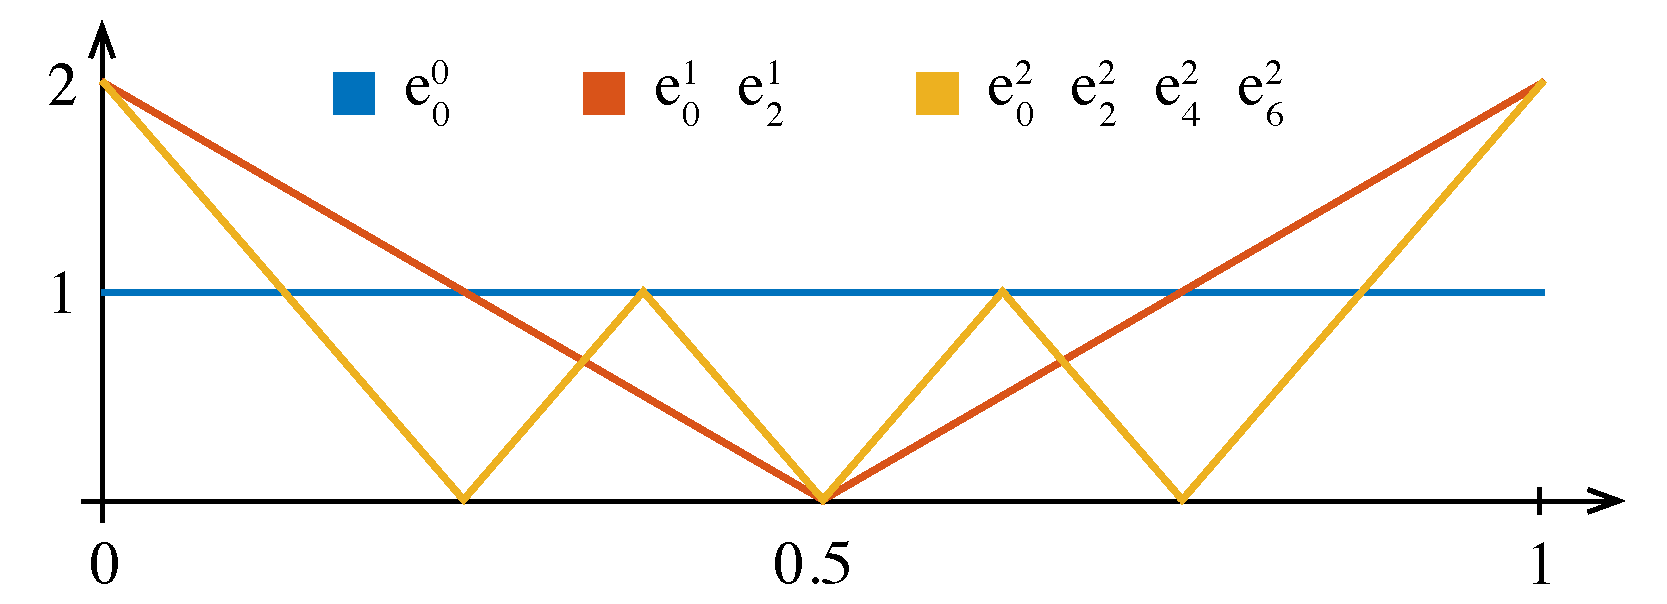
\includegraphics[width=1.0\columnwidth]{include/assets/basis.pdf}
  \caption{
    The basis functions, formed by the linear hat function, of the first three
    levels of interpolation.
  }
  \flab{basis}
\end{figure}

The basis functions are formed by the linear hat function and are as follows
\cite{klimke2006}. For $i = 0$ and $j = 0$,
\[
  \e^0_0(\x) = 1.
\]
For $i > 0$ and $j = 0$ (close to the left endpoint),
\[
  \e^i_0(\x) = \begin{cases}
    2 - \left( \n_i + 1 \right) \x, & \text{if } \x < \frac{2}{\n_i + 1}, \\
    0, & \text{otherwise}.
  \end{cases}
\]
For $i > 0$ and $j = \n_i - 1$ (close to the right endpoint),
\[
  \e^i_{\n_i - 1}(\x) = \begin{cases}
    \left( \n_i + 1 \right) \x - \n_i + 1, & \text{if } \x > \frac{\n_i - 1}{\n_i + 1}, \\
    0, & \text{otherwise}.
  \end{cases}
\]
In other cases,
\[
  \e^i_j(\x) = \begin{cases}
    1 - \left( \n_i + 1 \right)|\x - \x^i_j|, & \text{if } |\x - \x^i_j| < \frac{1}{\n_i + 1}, \\
    0, & \text{otherwise}.
  \end{cases}
\]
The basis functions corresponding to the first three levels of one-dimensional
interpolation are depicted in \fref{basis}. Note that $\e^1_1$, $\e^2_1$,
$\e^2_3$, and $\e^2_5$ are not depicted as they are not involved in the
hierarchical construction. In multiple dimensions, the basis functions are
formed as shown in \eref{basis-functions}.
